\message{ !name(fem.tex)}
\message{ !name(fem.tex) !offset(-2) }
\section{Método dos Elementos Finitos (FEM)}\label{fem}
A presente seção busca introduzir alguns dos importantes conceitos referentes ao Método dos Elementos Finitos (FEM). Busca-se balancear a exposição de conceitos fundamentais com uma maneira sintética de expor tais ideias de modo a ser conciso e didático. Para mais informações refere-se a \cite{langtangen2017}, livro base onde a estrutura da presente seção foi baseada.

O procedimento padrão para a modelagem matemática de fenômenos físicos parte de Leis Fundamentais da física (como as leis de conservação de massa, $\mathcal{M}$, momento, $\mathcal{P}$, e energia interna, $\mathcal{H}$) e de propriedades características representadas por equações constitutivas (como a Lei de Hooke em elasticidade linear e a Lei de Fourier em transferência de energia térmica). O presente trabalho envolverá a resolução de um sistema de equações diferenciais parciais resultantes de duas equações de conservação (são elas, conservação de massa, $\mathcal{M}$, e de energia interna, $\mathcal{H}$) e diversas equações de estado, entre elas as curvas de sorção isotérmicas, $\phi = f(P, T)$, a Lei de Fourier para a descrição do fluxo de calor, $\vec{q}_\mathcal{H} = - k \nabla T$ e a Lei de Darcy para a descrição do fluxo de massa, $\vec{q}_\mathcal{M} = -  \frac{\kappa}{\mu} \nabla P$ (Mais detalhes em \ref{modelos}).

As equações diferenciais são os objetos matemáticos mais importantes para a
representação matemática de fenômenos físicos inclusive existindo casos de
desenvolvimentos matemáticos (em termos de terminologia e técnicas de resolução)
resultantes de inspirações obtidas nos problemas físicos referentes a cada
conjunto de equações \cite{Zauderer2006}. A descrição de taxas temporais ou de
gradientes espaciais levam em consideração a ideia do efeito que um pequeno
diferencial em uma variável independente (tempo, dimensão em $x$, $y$, ou $z$)
tem em uma variável dependente (temperatura, campo elétrico, campo magnético, tensão mecânica, etc.), com isso permitindo a descrição de fenômenos no tempo e espaço (por exemplo, como varia a temperatura $T$ em um pequeno diferencial $\partial x$).

Tais equações podem ser classificadas em equações diferencias ordinárias (ODE) quando se tem apenas funções de uma única variável independente e suas derivadas, ou em equações diferencias parciais (PDE) quando se tem funções de várias variáveis independentes e suas respectivas derivadas parciais.

No geral, as ODE's lineares podem ser resolvidas analiticamente, isto é, é
possível obter sua solução em uma forma fechada (uma expressão matemática que
pode ser avaliada em um número finito de operações algébricas). Por outro lado, as PDE's muitas vezes exigem procedimentos de solução mais complexos, fazendo uso de expansões em séries, análises de similaridade e análises assintóticas. Uma grande
complicação de tais métodos é que em geral funcionam apenas para geometrias e
condições de contorno tão simplificadas ao ponto de se distanciar
consideravelmente da realidade.

Como alternativa a tais métodos e através do avanço da capacidade computacional
os métodos numéricos alcançaram uma elevada relevância. O desenvolvimento de
\textit{softwares} comerciais permitiram que tais métodos fossem popularizados
mesmo entre usuários que não possuem conhecimento dos detalhes da implementação
de tais metodologias. Naturalmente tais \textit{softwares} se especializaram em
análises mais populares como por exemplo cálculos de análises estruturais,
análises térmicas e fluído-dinâmicas. Dessa forma, casos mais específicos onde
se tem o acoplamento de situações relativamente incomuns (como o acoplamento do
transporte de massa e de energia necessárias ao presente trabalho) não são implementados.

Assim, justifica-se o desenvolvimento de um modelo através da metodologia dos elementos finitos, uma das mais comuns metodologias de solução de PDE's e ODE's através do uso de uma malha para representar domínios com geometrias complexas. Para tanto, utilizar-se-á o pacote FEniCS da linguagem Python. Como o desenvolvimento do modelo se dará desde a escolha do tipo de elemento, das funções de forma, nós de integração entre outros, é necessário revisar os conceitos fundamentais necessários para a implementação do modelo. Também espera-se que o presente texto sirva como uma breve introdução para os alunos iniciantes nessa metodologia.

	\subsection{Métodos de aproximação de funções}
	A metodologia por trás do FEM, é uma formulação já estabelecida que permite a
  aproximação de funções de uma maneira sistemática através de funções de forma
  sobre uma malha. De uma maneira mais detalha pode-se resumir a metodologia
  como:
  \begin{enumerate}
  \item Descritização do domínio em elementos finitos
  \item Derivação de equações sobre cada elemento da malha seguindo uma
    metodologia de aproximação
  \item Acoplamento das equações locais dos elementos resultando num sistema
    global de equações lineares
  \item Imposição de condições de contorno (ajustes nas matrizes e vetores)
  \item Solução numérica das equações
  \item Pós processamento dos resultados
  \end{enumerate}

  O software FEniCS \cite{AlnaesBlechta2015a} automatiza a grande maioria das
  etapas listadas, permitindo que o foco seja nas análises dos resultados e suas
  respectivas interpretações. Assim, a presente seção não abordará aspectos
  fundamentais (como a metodologia de acoplação do sistema global ou as
  metodologias de resolução numérica do sistema) mas automatizados dando enfoque
  para aspectos que ilustrem os conceitos lógicos por trás da metodologia (como
  as metodologias de aproximação, algumas funções de elementos finitos e as
  formulações variacionais). Com  tal introdução será possível justificar a
  escolha de parâmetros do modelo como o tipo de elemento, a malha utilizada, a
  formulação utilizada entre outros.
  
  Inicialmente criaremos intuição a partir das metodologias de aproximação, em
  especial o Método de Galerkin para poder derivar as equações locais de cada
  elemento. Existem inúmeras variações de tal metodologia, com alterações
  pontuais, recebendo nomes distintos, porém no presente trabalho o uso da
  metodologia de Galerkin será o suficiente.

  Antes de introduzir a metodologia para a obtenção de soluções numéricas de equações diferenciais, iniciaremos e definiremos objetos matemáticos a partir da aproximação de Galerkin para funções (de fato funções podem ser encaradas como vetores que residem em um espaço de dimensões infinitas e portanto, a aproximação de funções se equivale à aproximação de vetores). Isso tornará a metodologia mais palpável.

  \subsection{Aproximação de Galerkin}
  Para ilustrar a metodologia utilizaremos a aproximação de uma equação trivial: 
  \begin{equation}
  \uvec = \vvec 
  \end{equation}
    Tal equação representa a busca pela melhor aproximação do vetor $\vvec$, que
    reside no espaço vetorial $V$, através do vetor $\uvec$ existente em um
    subespaço de $V$. Existem duas abordagens para encontrar o melhor vetor $\uvec$ motivadas por conceitos da álgebra linear que nos permitem formalizar algoritmos para a resolução dessa tarefa, são elas a metodologia dos mínimos quadrados e a metodologia da projeção. Tais metodologias são descritas nas Definições \ref{def:minqua} e \ref{def:metproj} .

  \begin{Definition}{Metodologia dos Mínimos Quadrados}{minqua}
  A melhor aproximação de um vetor, $\vvec$ se dá quando o vetor erro $\evec =
  \vvec - \uvec$ (isto é a diferença entre o vetor $\vvec$ e a aproximação
  $\uvec$) possui a menor norma (a partir da métrica definida no espaço vetorial
  em questão) possível, isto é: $$\frac{\partial e}{\partial c_i} = 0 $$ para
  cada coeficiente $c_i$ de cada vetor base do subespaço do espaço vetorial $V$ que abriga $\uvec$.
  \end{Definition}

  \begin{Definition}{Metodologia da Projeção}{metproj}
  A melhor aproximação de um vetor, $\vvec$, se dá quando seu erro, o vetor $\evec =
  \vvec - \uvec$ é perpendicular (o termo mais geral seria ortogonal) ao subespaço ao qual o vetor $\vvec$ reside, isto é :$$ \evec \cdot \uvec = 0 $$
  \end{Definition}
  
  A metodologia proposta na Definição \ref{def:minqua} é bastante intuitiva,
  porém a metodologia da Projeção pode ser mais complicada de se visualizar.
  Para tanto,  na Figura \ref{fig:2dvecs} é possível observar como o menor erro
  entre  $\vvec$  e  $\uvec$ se dá quando o erro  $\evec$  é perpendicular ao
  espaço onde  $\uvec$ existe.  Observe que a aproximação da figura representa a
  aproximação de dois vetores existentes em um espaço Euclidiano representado em
  coordenadas Cartesianas, o  que poderá ser generalizado para vetores definidos
  em espaços de maiores, ou ainda de infinitas dimensões. Nesse contexto, como funções são vetores, pode-se garantir que ambas metodologias acima definidas também resultarão em  metodologias de aproximação de funções (que são vetores, afinal).

  \begin{figure}[ht]
	\centering
	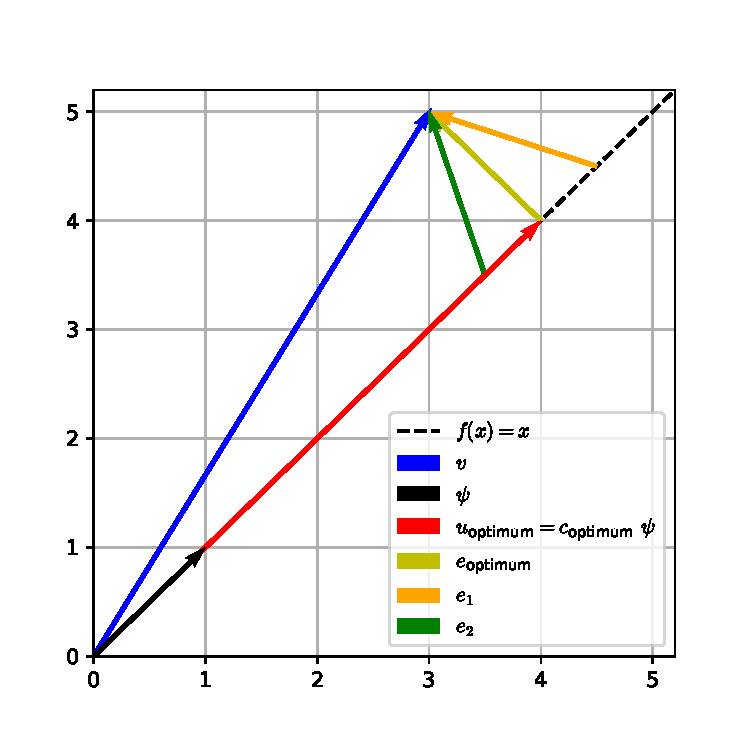
\includegraphics[width=\linewidth]{./figures/2dvectors.pdf}
	\caption{Representação da aproximação de vetores bidimensionais em coordenadas
    Cartesianas.  \label{fig:2dvecs}}
  \end{figure}

  É evidente que a melhor aproximação $\uvec_{optimum}$ resulta no erro de menor norma Euclidiana (comprimento do vetor, seguindo a definição de uma norma em um espaço vetorial Euclidiano), entretanto observe também que o erro ótimo, $\evec_{optimum}$ é perpendicular a reta onde reside o vetor $\uvec$ que estamos tentando aproximar. Lembrando-se da Geometria Analítica, quando dois vetores
  são perpendiculares seu produto interno é nulo.
  
 O russo Boris Galerkin usou o mesmo  princípio para obter a solução de equações
 diferenciais, definindo o método de Galerkin \cite{reddy1993introduction}.
  
	\subsection{Funções de forma}
	Como visto, anteriormente nos exemplos de vetores de duas dimensões no espaço
  Euclidiano, as aproximações de determinado vetor podem ser representadas
  através de combinações lineares de coeficientes e os vetores bases que definem
  o espaço vetorial. O que as metodologias de aproximação fornecem, são
  algoritmos que permitem encontrar o conjunto de coeficientes que formam a
  combinação linear dos vetores base cujo erro é o menor possível (dado uma certa métrica), segundo a Definição \ref{def:minqua} ou que o erro seja ortogonal ao subespaço ao qual o vetor a ser aproximado reside, segundo a Definição \ref{def:metproj}.

  	Assim, é evidente que a escolha dos vetores base é uma escolha primordial para que o processo de aproximação seja o mais prático possível. Dentre as várias possibilidades, é comum a busca por vetores ortogonais e isso pode ser mostrado pelo apelo que certas funções ortogonais apresentam como as funções trigonométricas seno e cosseno que são as bases das aproximações de Fourier.

  	No caso de tais funções trigonométricas seu domínio é o mesmo que todo o
    domínio ao qual a função a ser aproximada se estende, porém, uma estratégia
    que se pode utilizar é o uso de funções base com suporte compacto, isto é,
    funções que são não nulas apenas em uma porção do domínio, e zero em todo o
    resto do domínio, essas funções bases são as funções de elemento finito,
    usadas em FEM. A Figura \ref{fig:P1fun} ilustra uma função base de elementos
    finitos definida por partes e linear (referenciada no presente trabalho como
    $P_1$ \cite{arnold2014periodic}). Cada nó é associado com uma função desse tipo

  \begin{figure}[ht]
	\centering
	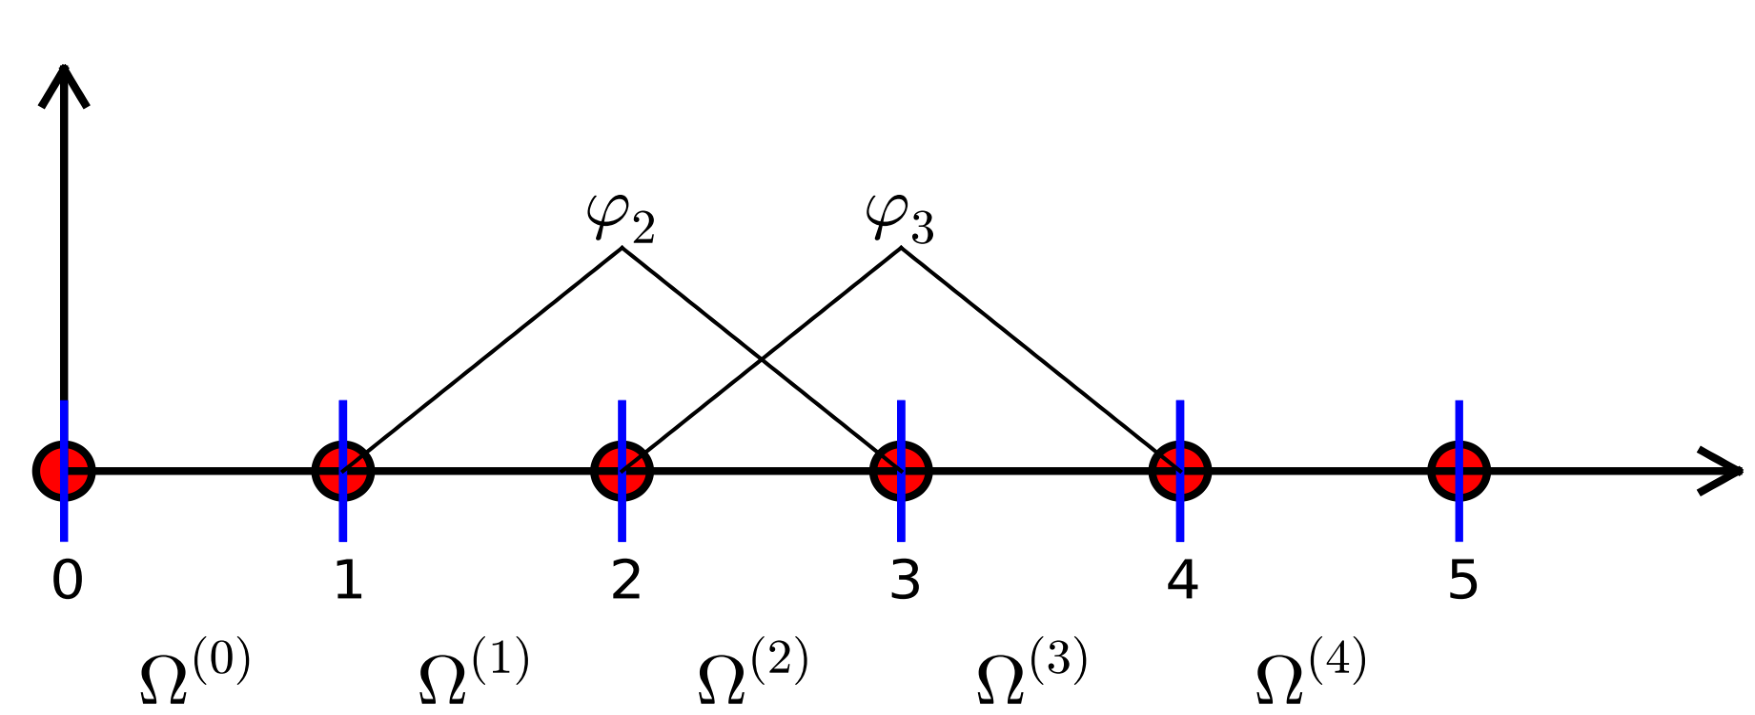
\includegraphics[width=\linewidth]{./figures/P1_fun.pdf}
	\caption{Representação de duas funções do tipo $P_1$, $\varphi_2$ e
    $\varphi_3$, em uma malha unidimensional com 5 elementos $\Omega^{(i)} $.  \label{fig:P1fun}}
  \end{figure}

  Tais funções são excelentes motivações para a divisão do domínio em uma malha,
  pois em cada elemento de determinada malha tem-se funções de forma que são não
  nulas nessa região do domínio. A vantagem é que se pode definir domínios
  complexos de uma maneira sistemática onde a convergência é obtida conforme a
  malha se torna mais refinada (isto é, com maior número de elementos
  representando o domínio) além de se obter, matrizes que são
  positivas-definidas durante a resolução numérica o que facilita tal processo.

    \subsubsection{Malha}
    	A malha é uma partição do domínio em elementos cuja intersecção é nula e cuja união resulta exatamente no domínio. O conceito mais generalizado de um elemento finito é apresentado na Definição \ref{def:elemento}.

    \begin{Definition}{Definição Geral de Elemento Finito}{elemento}
      \begin{itemize}
        \item Um elemento finito é uma célula em um sistema de coordenadas
      locais de referência cujos limites são chamados de vértices.

        \item Em cada célula se define um conjunto de funções base do tipo de elementos
      finitos e um conjunto de graus de liberdade, isto é, quantidades que se
      busca calcular (por exemplo, a temperatura em determinado ponto ao resolver
      a equação de calor).
     
        \item Finalmente define-se um mapa entre os graus de liberdade locais (de dentro
      do elemento) e os globais (definidos em todo domínio). Tal mapa serve para
      organizar os resultados obtidos após o cálculo. Além disso, define-se um
      mapa geométrico entre a célula e o domínio físico.
      \end{itemize}
      \end{Definition}

    A princípio pode-se parecer que tais definições acabem tornando o método apenas mais complexo e abstrato. Porém, tal abstração garante que a  metodologia de resolução no elemento seja feita individualmente elemento a elemento (inclusive usando o mesmo procedimento, pois usa-se o mesmo elemento de coordenadas de referência) sem considerar as especificidades referentes a geometria. Após o cálculo em cada elemento se realiza o processo de \textit{assembly} onde se une as informações de cada elemento obtendo os graus de liberdade em todo domínio.
    
    Uma vez definido a malha e os elementos a resolução do sistema de equações  pode ser montado a partir da forma variacional do problema. A seção seguinte traz o conceito de forma variacional.

    \subsection{Forma variacional}
    Para poder utilizar o método de Galerkin o problema precisa ser reformulado de uma maneira específica, chamada de "Forma Fraca" ou "Forma variacional". Essa reformulação é o "preço" a ser pago para poder resolver um problema definido em um espaço com dimensões infinitas (o espaço do problema físico em si, definido através das leis fundamentais e equações de estado) em um espaço de dimensões finitas (o subespaço onde se encontrará a solução).
    

\message{ !name(fem.tex) !offset(-179) }
